\begin{savequote}[75mm]
In that sense, this new knowledge has all to do with honor and country, but it has nothing to do directly with defending our country except to help make it worth defending. 
\qauthor{Robert R. Wilson during the Congressional Testimony on building Fermilab's first accelerator}
\end{savequote}


\chapter{The LHCb Experiment and its Upgrade}
\label{chapter:detector}
This chapter is split into two parts, and the first one is dedicated to present a detailed description of the LHCb detector that was deployed during both Run I and Run II.  This part starts by presenting the CERN (The European Organization for Nuclear Research). Then a basic understanding of how the LHC ( \textsc{Large Hadron Collider} works is explained. The mentioned section is followed by a description of the LHCb detector, which consists of a paragraph dedicated to each sub-detectors.  The final section discusses the LHCb Upgrade by presenting its motivation and summarizing all changes that have been planned. 

\section{CERN}
The European Organization for Nuclear Research CERN is the world's largest scientific organization in the field of High Energy Physics. It was established in 1954 by twelve western European countries to create one of the very first European joint ventures. Currently, the CERN associate 22 members state, including Poland. The Institution is based on the Swiss-France border very close to Geneva. The CERN's primary focus is to design and construct instruments to study the fundamental building of matter and its interactions.  

\begingroup
    \expandafter\patchcmd\csname Gin@ii\endcsname   % needed etoolbox
      {\setkeys {Gin}{#1}}
      {\setkeys {Gin}
          {width=\linewidth,                     % standard graphicx settings
           valign=c, margin=-3pt 6pt 0pt 6pt,#1}     % settings from adjustbox
      }
      {}{}

\section{Large Hadron Collider}
The Large Hadron Collider (LHC) is the world's largest circular particle accelerator. It is installed in the 26.7 km long tunnel that was constructed for the previous experiment, Large Electron Positon Collider (LEP) \cite{lep}. The tunnel is situated about 100 m below the ground. 
The LHC is designed to accelerate the protons and heavy ions. At the nominal performance, the LHC delivers the two protons beams of energy 6.5 TeV.  This corresponds to the center-of-mass collision energy of 13 TeV. 
To achieve this performance, the particle acceleration is done by a series of accelerators. Each of them progressively boosts the energy of the beam. Figure \ref{fig:LHC} shows the LHC accelerator complex. 

\begin{figure}
\centering
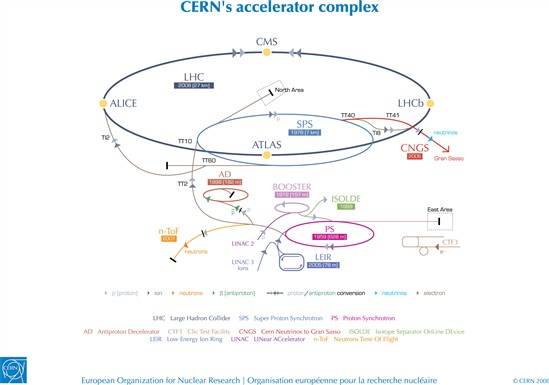
\includegraphics{figures/LHC.jpg}
\caption{The LHC accelerator complex showing all accelerator facilities and the four main experiments. Figure adapted from \cite{LHC_complex}
\label{fig:LHC}}
\end{figure}

The entire boosting process starts from the small red bottle full of hydrogen. It is shown in figure \ref{fig:Bottle}. This bottle is the only and sufficient proton source for the entire, massive LHC acceleration system. This shows how sophisticated and resource-efficient LHC is. Then, the hydrogen atoms are ionized by the external electric field to yield the protons. These particles are injected into the Liniac2, the first linear accelerator in the chain, to boost its energy to the 50 MeV. After that, the beam is inserted into the Proton Synchrotron Booster, followed by the Proton Synchrotron (PS), which pushes the beam to the energy of 25 GeV. The next step in the acceleration sequence is performed by the Super Proton Synchrotron (SPS). It accelerates the beam to the energy of 450 GeV. \footnotes{The beam form SPS was used during the testbeam experiments, which is the topic of chapter \ref{chapter:testbeam}.} 

The protons are finally injected into two beam pipes of the LHC. The beam in one pipe circulates clockwise while the beam in the second pipe circulates anticlockwise. It takes 4 minutes and 20 seconds to fill each LHC ring, and 20 minutes for the protons to reach their maximum energy of 6.5 TeV. The two beams interact inside four detectors – ALICE \cite{Alice}, ATLAS \cite{Atlas}, CMS \cite{CMS}, and LHCb.

\begin{figure}
\centering
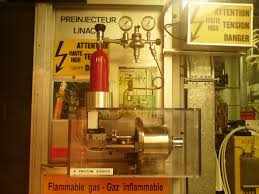
\includegraphics[scale=0.6]{figures/Bottle.jpg}
\caption{The LHC proton source 
\label{fig:Bottle}}
\end{figure}

One of the key parameters that describe a particle accelerator (note, that we consider here the circular machine), except for beam energy, is the quantity called instantaneous luminosity.  This quantity expresses the ability to produce the required number of interactions by an accelerator, and formally it is the proportionality factor between the number of events per second (also called the event rate) $\frac{dN}{dt}$ and the interaction cross-section $\sigma$:
\begin{equation}
   \frac{dN}{dt} = L \times \sigma 
\end{equation}
The unit of the luminosity is $cm^{-2}s^{-1}$.
In practice, the integrated luminosity $\mathcal{L}_{int}$ is often used. Based on this quantity, one can estimate the number of expected events for a given process.  

The relationship between the luminosity and the beam parameters for a circular machine, assuming that the beam profile is distributed according to the Gaussian distribution, and there is negligible energy loss during the bunch-bunch collisions is given by:

\begin{equation}
    L = \frac{N_{b}^2 \cdot n_b  \cdot f_{rev}  \cdot \gamma_{r}}{4 \pi \cdot \epsilon_n  \cdot \beta^* }  \cdot F
\end{equation}

where $N_b$ is the number of particles per bunch, $n_b$ the number of bunches per beam, $f_{rev}$ is the revolution frequency, $\gamma_{r}$ is the relativistic gamma factor, $\epsilon_n$ the normalized transverse beam emittance, $\beta^*$ the beta function at the  collision point, and $F$ the geometric luminosity reduction factor which originates from the crossing angle at the interaction point. 


The LHC was built to deliver a peak luminosity of $10^{34} cm^{-2}s^{-1}$ by colliding 2808 bunches containing approximately $1.1 \cdot 10^{11}$ protons per bunch with the bunch crossing rate of 40MHz (also called the machine clock).  For more details on the LHC machine, see \cite{LHC_machine}.

Figure \ref{fig:Luminosity} presents the integrated luminosity delivered to each of the LHC experiments. It is visible that LHCb operates at a significantly lower luminosity level that the remaining general-purpose experiments.  The LHCb detector was designed to operate at a luminosity of $2 \cdot 10^{32}cm^{-2}s^{-1}$, which is about two orders of magnitude less than the luminosity delivered to ATLAS and CMS experiments. This is done by purpose since the LHCb experiment focuses primarily on precision, indirect measurements. Operating at a lower luminosity produces fewer interactions, or primary vertices (PVs), per bunch crossing. An increasing number of PVs produce complications in physics analysis, such as tracks being identified coming from the wrong PV.  Moreover, operating at lower luminosities induces less radiation damage in the detectors operating very close to the proton beam. The LHCb collaboration implemented the luminosity levelling technique, described in \cite{lumi_down}, to meet the occupancy requirement. 

\begin{figure}
\centering
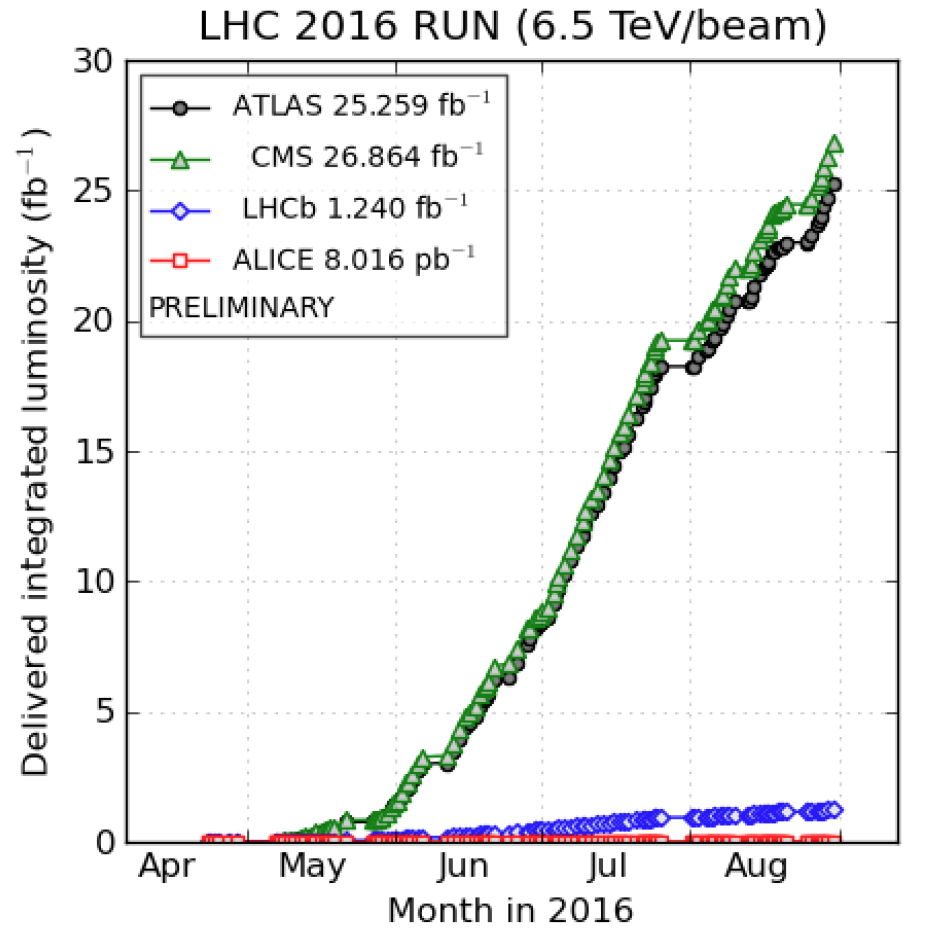
\includegraphics[scale=0.5]{figures/Luminosity.png}
\caption[Luminosity]{The integrated luminosity delivered to LHC experiments
\label{fig:Luminosity}}
\end{figure}


\section{LHCb detrctor}

The heart of the LHCb experiment is its detector. It was built to produce proton-proton collisions at a centre-of-mass energy of $\sqrt{s}=$14 TeV. It is located in the cavern that previously was used to host the LEP's experiment Delphi \cite{deplhi}. The unique feature of the LHCb detector is its design. It is significantly different from other general-purpose detectors like Atlas or CMS, which look like multi-layer barrels surrounding the collision point (so-called $4 \pi$ geometry).
On the contrary, the LHCb is a forward single-arm spectrometer, that was designed to cover the pseudorapidity range of $2< \eta < 5 $  \cite{lhcb}. The pseudorapidity is a spatial coordinate describing the angle of a particle relative to the beam axis. The  pseudorapidity can be calculated from the following formula: 

\begin{equation}
    \eta = - \ln\left[ \tan \left( \frac{\theta }{2}\right) \right]\nonumber = \frac{1}{2} \ln \left( \frac{|\vec{p}|+ p_t}{|\vec{p}|- p_t}  \right)
    \label{eq:eta}
\end{equation}

where $\theta$  is the angle between a particle's three-momentum $\vec{p}$ and the positive direction of the beam axis. The $p_t$ (transverse momentum) is a component of the $\vec{p}$ transverse to the beamline.
Equation \ref{eq:eta} allows finding the relationship between the parameter $\eta$ and the angle $\theta$. When the angle $\theta$ gets smaller, then the $\eta$ rises.


The choice of such layout was motivated by the LHCb physics programme, particularly the angular distribution of the $b \overline{b}$ pairs produced by proton-proton interactions at the LHC energies, fly predominantly into the forward and backward cones (see figure \ref{fig:bb}). LHCb geometrical coverage corresponds to only 4\% of whole solid angle, but it can detect approximately 25\% of all produced beauty hadrons. 

\begin{figure}[h]
 \begin{center}
  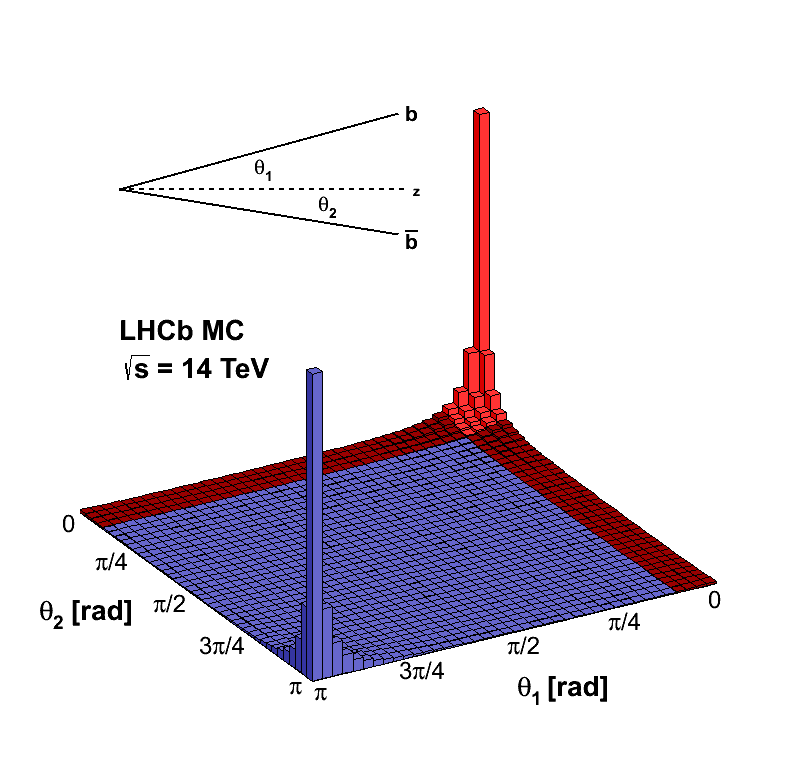
\includegraphics[width=0.48\linewidth]{figures/bb_2.png}
   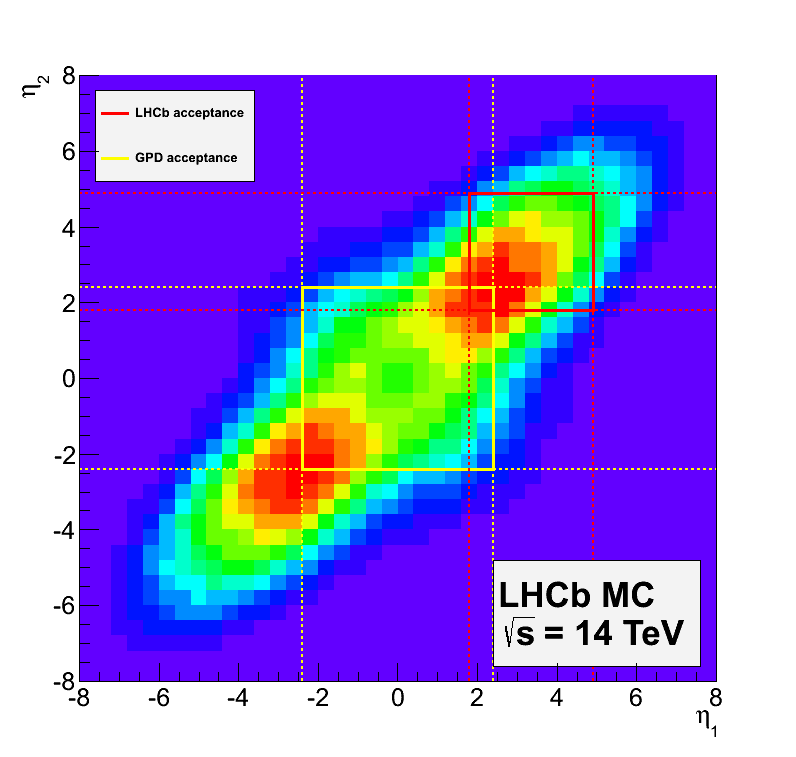
\includegraphics[width=0.48\linewidth]{figures/bb_1.png}
   \caption{Production of  $b \overline{b}$ quarks at LHC at 14 TeV. The left plot presents the production of the $b \overline{b}$ quarks as a function of polar angle $\theta$. The right plot shows the same distribution as a function of the rapidity of each quark. The pseudorapidity region inside a yellow square corresponds to the acceptance region of the Atlas and CMS detectors, while the red box highlights the acceptance region of LHCb. The figure is taken from \cite{bbangles}. 
     \label{fig:bb}}
 \end{center}
\end{figure}

The LHCb, like all of the currently operating High Energy Physics experiments, consists of several sub-detectors, each of which was carefully designed to provide highly efficient system, capable of detecting physics phenomena beyond the Standard Model (BSM). To correctly identify and reconstruct the decays and their kinematical properties, the LHCb detector needs to provide an excellent vertex reconstruction precision, momentum resolution, and particle identification. The following section is dedicated to describing each of the sub-systems.

\subsection{LCHb tracking sub-system}
\label{sec:lhcb_tracking_subsystem}
The tracking system was designed to reconstruct the trajectory of charged particles by combining information from a set of tracking stations. The reconstructed track information is used to estimate the momentum of the charged particles. This estimation is possible due to the magnet's installation, which creates a magnetic field used to bend a particle trajectory. The LHCb tracking system is composed of the Vertex Locator (VELO), the Tracker Turicensis (TT), and the three tracking stations T1, T2, and T3; see \ref{fig:LHCBlayout}.  The brief description of each tracking sub-detectors is a topic of this subsection. 

\subsubsection{Velo}
\label{sec:velo}
The Vertex Locator (Velo) \cite{VELO} is a silicon strip detector that is located close to the proton-proton collision point, and it is dedicated to providing precise measurements of the position of the primary and secondary vertices \footnote{The secondary vertex is a point of decay of short-lived particles, which was created in the primary interactions. }, which are essential to identify $b$ and $c$ hadrons, which typically traverse about 1 cm at LHCb.  
The Velo active area is just about 8 mm away from the beamline, which is the world record. Additionally, the Velo allows measuring the Impact Parameter of charged particle's trajectories. Impact Parameter is a transverse distance of closest approach between a particle trajectory and a vertex, most commonly the primary proton-proton interaction vertex, see figure \ref{fig:IP}. The Impact Parameter is widely used in many LHCb data analysis to make a selection that significantly reduces the contamination from the light-quark backgrounds.  


\begin{figure}[h]
\centering
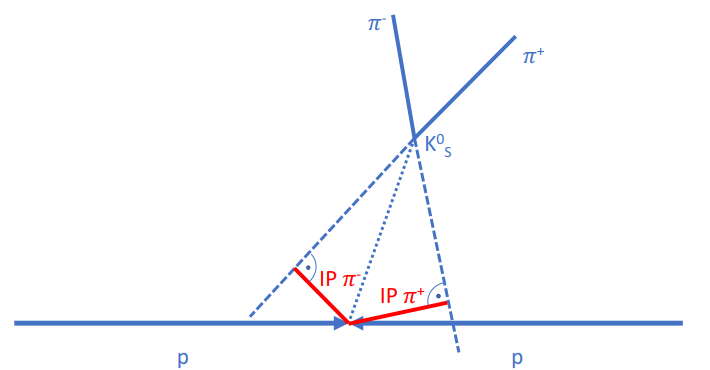
\includegraphics{figures/IP.PNG}
\caption{Graphical interpretation of the Impact Parameter (denoted in red). Figure presents a topology of the $K_S^0$ decaying to two pions.  
\label{fig:IP}}
\end{figure}

The Velo detector is comprised of twenty-one silicon tracking stations positioned along the beam axis ($z$-axis). Each of the tracking stations is divided into two retractable halves, called modules, each consisting of two silicon microstrip sensors. Figure \ref{fig:veloLayout} presents the layout of the Velo detector. All Velo sensors operate in the vacuum. The Velo vacuum is separated from the beam vacuum by a thin aluminium layer called RF foil.

\begin{figure}[h]
\centering
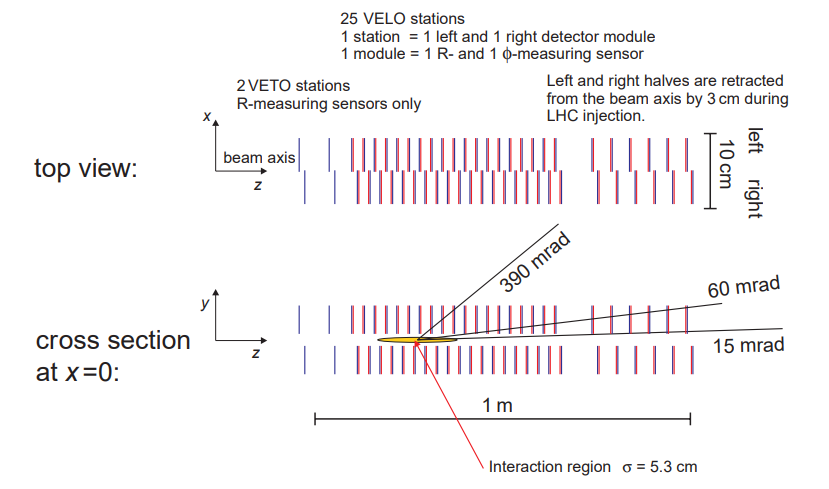
\includegraphics{figures/VeloLayout.png}
\caption{The layout of the Velo detector. The top picture presents the Velo setup seen from the top, indicating the overlap between the left and right detector's halves. The bottom figure is a cross-section of the Velo at $x=0$. The black lines indicate the maximum and minimum angular coverage of the Velo and the average angle of the tracks. The figure was taken from \cite{VELO}. 
\label{fig:veloLayout}}
\end{figure}

The first type of the Velo sensor is called $R$-type, and it is dedicated to measuring $r$-coordinate, i.e., the distance from the proton beam, thus, the strips have a semi-circular shape. The $R$-type sensors are divided into four sectors in the azimuthal angle to improve the pattern recognition phase of the track reconstruction. The strip pitch \footnote{Pitch is a distance between the centres of two adjacent strip implants} increases from $38\mu m$ at the innermost region to $102 \mu m$ at the far edge. The $\varphi$-type sensor is, in turn, divided into two regions, inner and outer, with different pitches to cope with high occupancies. The respective strip topologies are presented in Figure \ref{fig:velo}. Both $R$ and $\varphi$ sensors have a thickness of $300 \mu m$. The Velo sensors and read-out electronics are cooled by the evaporated $CO_2$ system. This system keeps the sensors approximately at the temperature of $-8^\circ$C during data taking.  

\begin{figure}[h]
 \begin{center}
  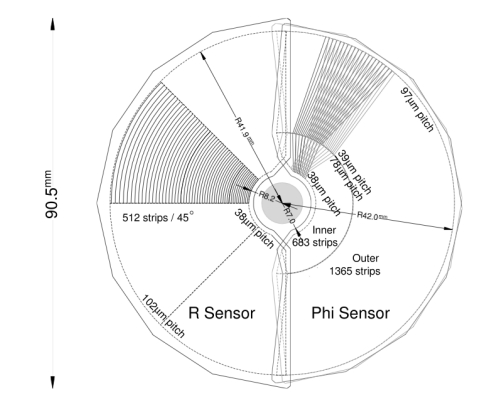
\includegraphics[width=0.8\linewidth]{figures/VeloGeometry.PNG}
   %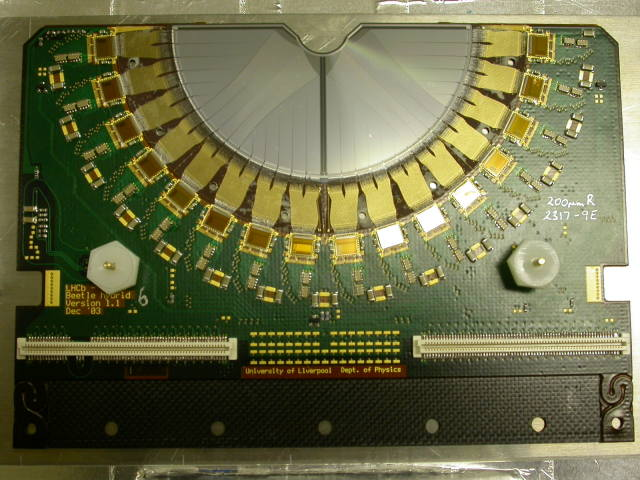
\includegraphics[width=0.4\linewidth]{figures/Velo_photo.jpg}
   \caption{Geometry of the Velo $R$ and  $\varphi$ sensors, with only a small portion of strips visible for clarity (left). 
   %The photo of the Velo module with 16 readout Beetle chips (right). 
   Figure was taken from\cite{lhcb}.  
     \label{fig:velo}}
 \end{center}
\end{figure}

The read-out of the data is performed by the Beetle front-end ASIC\footnote{ASIC stands from Application-specific integrated circuit}\cite{Beetle}. These chips are placed on the outer edge of the sensor, see figure \ref{fig:velo1}. The Beetle chip integrates 128 channels with low-noise charge-sensitive preamplifiers and shapers, an analogue pipelined memory, and a multiplexer.

\begin{figure}[h]
 \begin{center}
   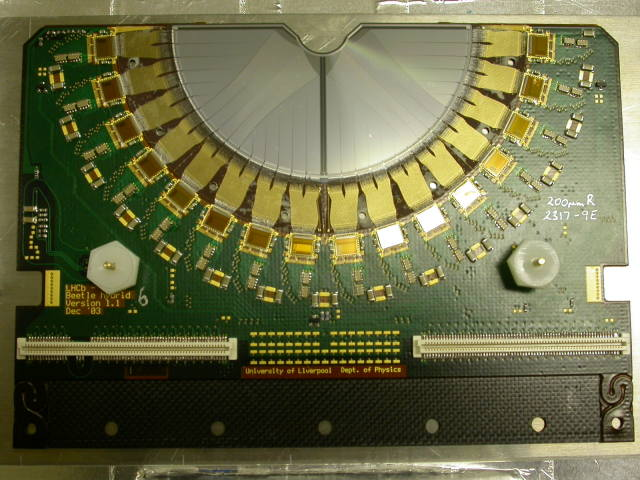
\includegraphics[width=0.6\linewidth]{figures/Velo_photo.jpg}
   \caption{
   The photo of a Velo module with 16 readout Beetle chips (right). 
   Figure was taken from\cite{lhcb}.  
     \label{fig:velo1}}
 \end{center}
\end{figure}

The primary vertex spatial resolution of about $13 \mu m $ in the transverse plane and close $70 \mu m $ along the $z$ axis allows for very precise decay-time measurements that are vital for the LHCb physics programme. The dependence of the primary vertex resolution versus number of tracks obtained using 2012 calibration data is shown in figure \ref{fig:veloPerformance}. The resolution of the Impact Parameter, critical for detecting the displaced secondary 
heavy-flavour decay vertices, depends on  multiple scattering, primary vertex resolution and single-hit resolution can be expressed as a function of transverse momentum $p_t$ \cite{veloPerformance}: 

\begin{equation}
    \sigma_{IP} = \left( 11.5  + \frac{24.5}{p_t[GeV/c^2]} \right)
\end{equation}

\begin{figure}[h]
\centering
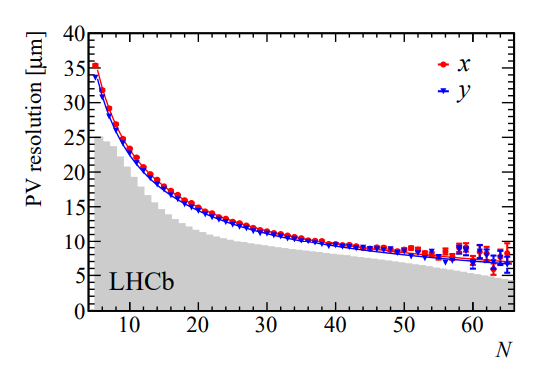
\includegraphics{figures/VeloResolution.PNG}
\caption{Primary vertex resolution as a function of a track multiplicity. The blue curve corresponds to $x$ coordinate of the Primary Vertex, and the red one to the $y$ coordinate. The gray histogram presents the number of tracks per reconstructed primary vertex. Presented results were obtained using 2012 calibration data with only one reconstructed primary vertex in the event. Figure taken from \cite{veloPerformance} 
\label{fig:veloPerformance}}
\end{figure}

\subsubsection{Silicon Tracker}
\label{sec:ST}
Silicon Tracker \cite{Silicon_Tracker} sub-system consists of two detectors based on similar technology; the TT (Tracking Turicensis), upstream to the magnet, while the IT (Inner Tracker) is a part of the tracking stations (T1, T2, T3, see figure \ref{fig:LHCBlayout}) located downstream to the magnet.

The primary purpose of the TT detector is to reconstruct low-momentum tracks and decays of the long-lived particles, which decay outside of the Velo. The IT detector reconstructs tracks with momentum larger than $1.5 GeV/c$, near the beam axis, that passed through the magnetic field. It covers approximately $2\%$ of the T stations acceptance, which corresponds to $20\%$ of all tracks that pass through this detector. On the other hand, TT is designed to cover the full LHCb acceptance region.  

Both TT stations (TTa and TTb) are composed of two measuring planes capable of providing a 3d space point for each particle hit. By convention, the sensitive planes are denoted as $(TTaX, TTaU, TTbV, TTbX)$. The $X$ coordinate is measured in the direction perpendicular to the direction of TT sensor vertical strips. Coordinates $U$ and $V$ are identical to the $X$ but tilted  by $-5^{\circ}$ and $5^{\circ}$ respectively (see Figure \ref{fig:TT}). The distance between the two adjacent layers within each station is about 4 cm, and the distance between the TTa and TTb stations is 27 cm. The TT silicon sensors (p-on-n) are $500 \mu m$ thick with a constant strip pitch of $183 \mu m$.  

\begin{figure}[h]
 \begin{center}
  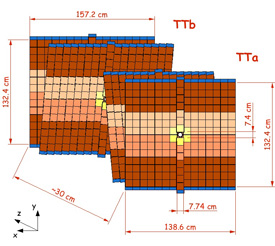
\includegraphics[width=0.49\linewidth]{figures/TT-layout.jpg}
   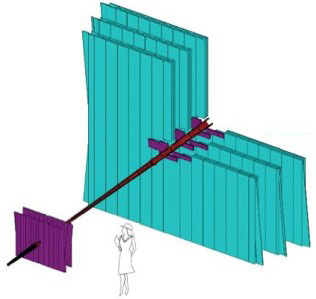
\includegraphics[width=0.49\linewidth]{figures/Tracking-system-diagram-2.jpg}
   \caption{The layout of the TT station (left) and the schematic view of the whole ST system (plotted in magenta), the cartoon of the woman is shown to indicate the size of each detectors (right). Figure taken from \cite{lhcb}.  
     \label{fig:TT}}
 \end{center}
\end{figure}

One of the quantities that can be used to determine ST performance is the hit efficiency, which can be expressed as a ratio between the number of measured hits to the number of hits expected in a given region. This ratio was measured to be $99.7\%$ for TT and $99.8\%$ for the IT. This measurement was performed on the data collected during Run 1. Another important metric to determine ST performance is the hit spatial resolution.  For 2012 the hit resolution was measured to be $53.4 \mu m$ for the TT and $54.9 \mu m$ for IT.  


\subsubsection{Outer Tracker}

 The Outer Tracker (OT) \cite{OT} is a complementary element to the IT detector, designed to cover the remaining LHCb acceptance region. Each of the OT modules is made of drift-time straw tubes filled with a gas mixture of $70\%$ of Argon and $30\%$ of $CO_2$. 
The Drift-time detector reconstructs the hit position by measuring the drift time of the ionization electron to the anode located at the centre of the tube. The distance between the wire and the particle's trajectory is determined by comparing the drift time with bunch crossing signals.  The ionization electron is created when a charged particle interacts with a gas. OT achieves drift time less than $50 ns$, which allows reconstructing hits with a spatial resolution of $200 \mu m$. OT has a consistent layout of the IT detector, which means it also has four modules in  $(X, U, V, X)$ orientation, which is shown in figure \ref{fig:OT}. 


\begin{figure}[!hb]
\centering
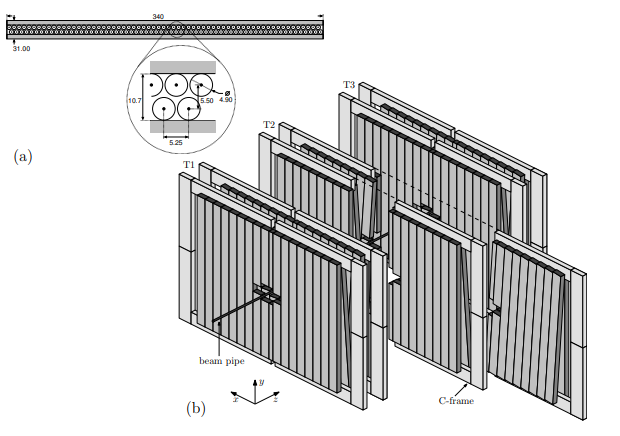
\includegraphics[scale=0.7]{figures/OT.PNG}
\caption{Schematic view of the OT stations. Figure (a) presents the cross-section of a single OT module, all distances are given in $mm$, and the arrangement of OT modules in layers and stations around the beam pipe (b).  Figure was taken from \cite{lhcb}.
\label{fig:OT}}
\end{figure}

\subsubsection{Magnet}

The LHCb Magnet plays a crucial role within the experiment. It bends the trajectory of the charged particles allowing to estimate its momentum. LHCb detector is equipped with a single warm dipole magnet. The magnet is situated between TT and T tracking stations. 
Figure \ref{fig:magnet} shows a photography of the Magnet. It is composed of two identical saddle-shaped coils. These coils are placed inside an iron yoke, that is compatible with the acceptance of the LHCb detector. The coils are made of AI-99.7 alloy with a 25 mm diameter central channel for water cooling. 

The estimated momentum resolution depends on the proper measurement of the magnetic field. Therefore, a careful procedure to measure the magnetic field was conducted. As the outcome, the precision of the measurement of the magnetic field is quoted to be $4 \cdot 10 \%{-4} \delta B /B $, and the maximal magnitude is 1.04 T, which is shown in figure \ref{fig:magnet}. 

The systematic errors related to the track reconstruction procedure, which can play a dominant role in the precise measurement of $CP$ asymmetries,  can be decreased by operating the magnet at two polarities (positive and negative curves in figure \ref{fig:magnet}). The amount of data collected is approximately equal for both polarities, and this split can be used to cross-check systematic reconstruction effects.

\begin{figure}[h]
 \begin{center}
  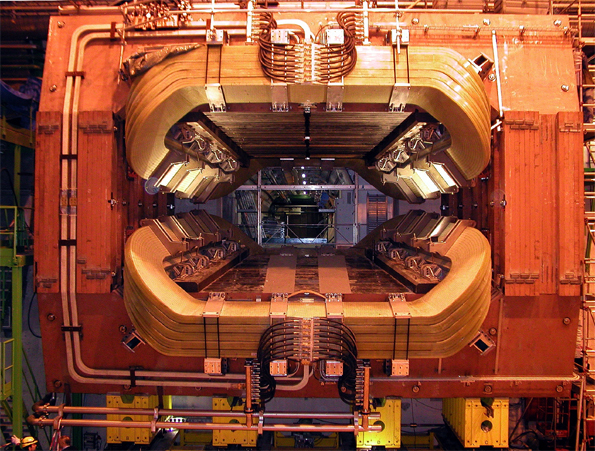
\includegraphics[width=0.49\linewidth]{figures/magnet_photo.jpg}
   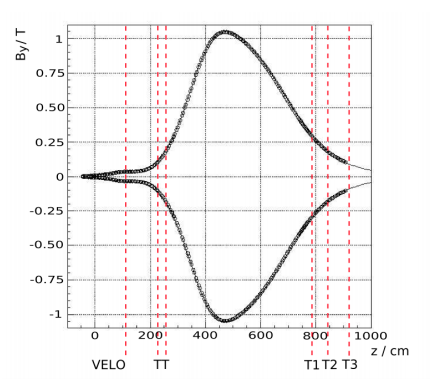
\includegraphics[width=0.49\linewidth]{figures/magnet_profile.PNG}
   \caption{A photo of the LHCb Magnet taken after its completion in 2004 is shown on the left-hand side. The picture was taken towards the direction of the Velo detector before other sub-detector have been installed, the visible parts are coils (yellowish) and yoke (reddish). Magnetic field profile as a function of the $z$ axis (direction along the beam pipe) is plotted on the right-hand side. The red dashed lines correspond to the location of the tracking sub-detectors (right). Figure taken from \cite{lhcb}.   
     \label{fig:magnet}}
 \end{center}
\end{figure}


\subsection{Particle identification}

Particle identification (PID) is a vital step in any physics analysis. For instance, the ability to significantly reduce the background often relies on the correct separation of kaons and protons from pions. The LHCb PID system is complex and comprises of two ring-imaging Cherenkov detectors (RICH), a series of muon chambers, and a calorimeter system (ECAL and HCAL), see figure \ref{fig:LHCBlayout}. 

The combined information from these sub-detectors allows distinguishing between various types of charged and neutral particles. Identification of the charged particles can be enhanced using tracking information. Calorimeters, apart from measuring the energy, can also provide information regarding the particle type for electrons, photons and hadrons. The muon system provides identification of muons with a high purity that is necessary for all CP-sensitive decay processes. Ability to distinguish pions and kaons/protons with high efficiency is done using the RICH detectors and is critical for the purely hadronic decays. It is important to note that for LHCb experiment the performance of the PID reconstruction is measured using data-driven techniques since the simulation poorly reproduces the PID variables. At the moment, two mutually exclusive approaches are used where simple low-level variables measured by respective sub-detectors are combined to provide more powerful selection variables. The first method, called $DLL_{X,\pi}$, relies on a linear combination of likelihood information produced by each detector which is then added to form the combined likelihood ratio (or difference of log-likelihoods) between particle $X$ (where $X \in {K, p, \mu, e}$) and pion hypothesis. So, the general idea of applying the $DLL_{X,\pi}$ method is to evaluate log-likelihood difference between a given particle $X$ and a pion hypothesis as follow:

\begin{equation}
\Delta log \mathcal{L}_{X,\pi} = log \mathcal{L}_{X} - log \mathcal{L}_{\pi}  
\end{equation}
Where: $ \mathcal{L}_{X}$ and $ \mathcal{L}_{\pi}$ represents log-likelihoods for particle $X$ and a $\pi$. The classification is performed by simply comparing the $DLL_{X,\pi}$ to a tuned threshold. When the $DLL_{X,\pi}$ is greater than this threshold, it means that the particle is likely not to be a pion. 


To enhance the PID performance the LHCb collaboration decided to apply also the multivariate analysis \cite{PID}. The model, called $ProbNNX$, that was proposed and deployed is a fully-connected neural network (that kind of model is described in section \ref{sec:DNN}) with one hidden-layer implemented using the TMVA package \cite{TMVA}. In order to produce the $ProbNNX$ output the tracking information, such as track momentum and pseudo-rapidity, is also used. In the end the output of the model is employed to distinguish a given particle specie $X$ from any other (i.e., a multi class classification problem). Additional models are trained to identify neutral particles as well. In particular two models $isNotE$ and $isNotH$ are trained to separate photons from electrons and hadrons respectively.
These baseline models proved that the application of Machine Learning could significantly improve the performance of Particle identification. Figure \ref{fig:PID baseline} shows performance comparisons using ROC curves \footnote{For a formal definition of ROC curve see section \ref{sec:ROC}} determined for respective models.

\begin{figure}[h]
 \begin{center}
  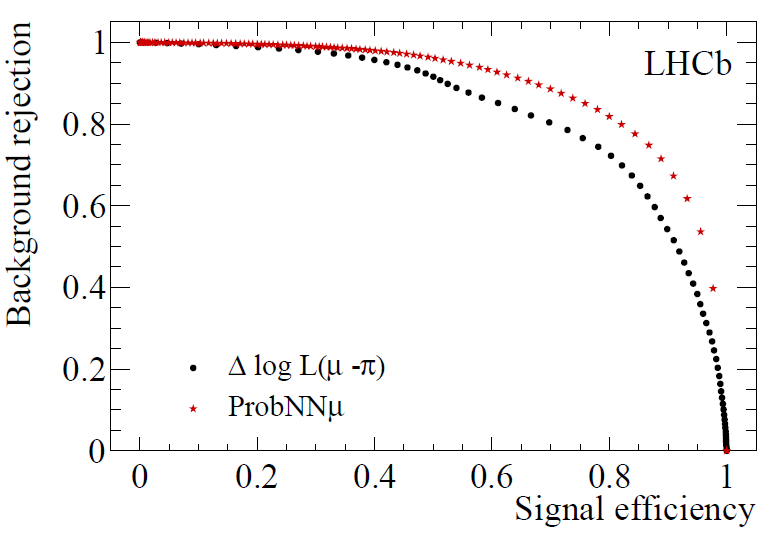
\includegraphics[width=0.49\linewidth]{figures/PID_prob_left.PNG}
   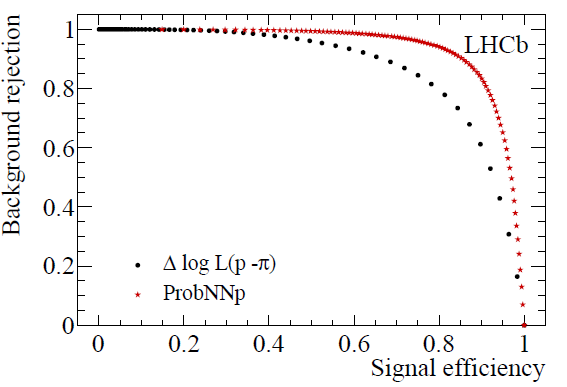
\includegraphics[width=0.49\linewidth]{figures/PID_prob_right.PNG}
    \caption{Background misidentification rates versus muon (left) and proton (right)
identification efficiency. The variables $\Delta \mathcal{L} (X −\pi)$
(black) and ProbNN (red), are compared for 5 − 10 $GeV\/c$ muons and 5 − 50 $GeV\/c$ protons,
using data sidebands for backgrounds and simulated samples for the signal. The data sample
used corresponds to 2012 sample collected at center-of-mass energy 8 GeV. Figure adapted from \cite{PID}}%
\label{fig:PID baseline}%
 \end{center}
\end{figure}

The overall Particle Identification performance can be summarize using the following figures of merit:

\begin{itemize}
    \item Electrons: $90\%$ identification efficiency with about $5\%$ electron to hadron missidentification probability. 
    \item Kaons: identification efficiency averaged over the momentum range of\\ $2-100~ GeV/c$ is $95\%$ with a nearly $5\%$ pion to kaon missidentification rate. 
    \item Muon: $97\%$ identification efficiency with pion to muon missidentification rate in between $1$ and $3\%$.  
\end{itemize}


The remainder of this section is dedicated to present each component of the Particle Identification system.


\subsubsection{RICH detector}

The most critical component of the Particle Identification system is the Ring Imaging Cherenkov detector (RICH). LHCb has two of these detectors installed \cite{RICH_performance}. The first one, called RICH1, is placed just before TT detector and the second one (RICH2) after T stations, see \ref{fig:LHCBlayout}. These detectors were designed to identify charged hadronic particles over a large momentum range of $2-100~ GeV/c$. To accomplish this task, RICH1 was filled $C_4F_{10}$ gas radiator, which provides sensitivity for particles with momentum in range $2-10~ GeV/c$ (low-momentum particles) including those that are swept out of the detector acceptance by the magnetic field. In contrast, RICH2 is filled with $CF_4$, which can be used to cover the momentum range of $15-100~ GeV/c$. The geometry of both RICH1 and RICH2 detectors are presented in figures \ref{fig:RICH1} and \ref{fig:RICH2}, respectively. 


\begin{figure}[h]
 \begin{center}
  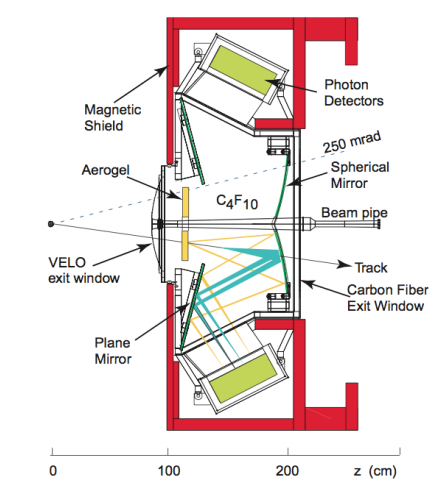
\includegraphics[width=0.49\linewidth]{figures/RICH1.PNG}
   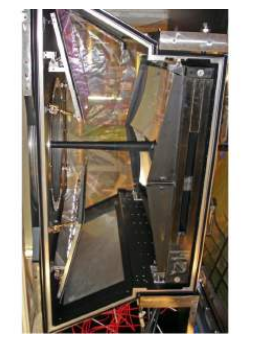
\includegraphics[width=0.49\linewidth]{figures/RICH1_photo.PNG}
    \caption{Geometry of the low momentum RICH detector (left), photo of the RICH1 detector (right). Figures taken from \cite{lhcb}}%
\label{fig:RICH1}%
 \end{center}
\end{figure}


\begin{figure}[h]
 \begin{center}
  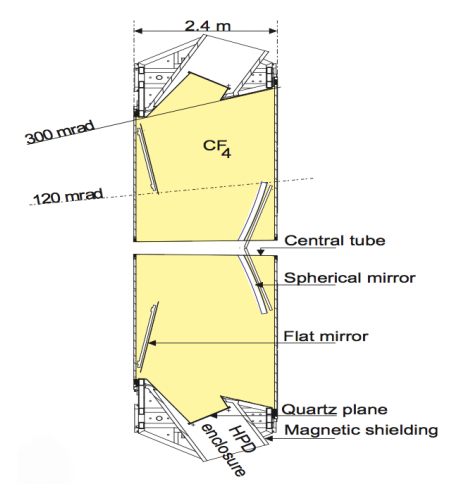
\includegraphics[width=0.49\linewidth]{figures/RICH2.PNG}
   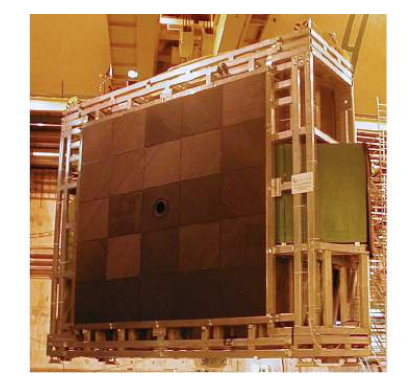
\includegraphics[width=0.49\linewidth]{figures/RICH2_photo.PNG}
    \caption{Geometry of the high momentum RICH detector (left), photo of the RICH2 detector (right). Figures taken from \cite{lhcb}}%
    \label{fig:RICH2}%
 \end{center}
\end{figure}

The fundamental principle of operation of the RICH detector is to measure Cherenkov radiation emitted when a charged particle traverses its active volume. Cherenkov radiation is always emitted when a charged particle moves through a medium at the velocity higher than the speed of light at this medium. The angle at which the Cherenkov photons are emitted ($\theta_c$) depends directly on the particle velocity, and it is expressed by

\begin{equation}
cos \theta_c = \frac{1}{n\beta}
\end{equation}

Where: $\beta$ is the velocity of the particle divided by the speed of light,\\ and $n = \frac{c}{v_{medium}}$
is the refractive index. 

Once emitted, Cherenkov radiation is reflected via a combination of spherical and flat mirrors to hybrid photon detectors (HPD). The HPD has a photocathode that emits electrons when excited by the Cherenkov radiation. Electrons are accelerated by a potential of about 20kV towards a silicon detector, which allows identifying the location of the hit. The performance, quantified using the identification efficiency is shown in figure \ref{fig:RICH_performance}. 


\begin{figure}[h]
 \begin{center}
  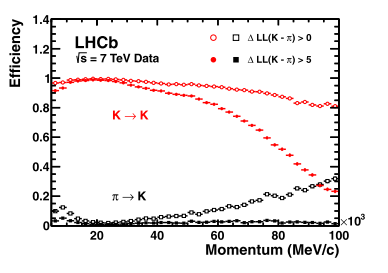
\includegraphics[width=0.49\linewidth]{figures/Kaon_proton.PNG}
   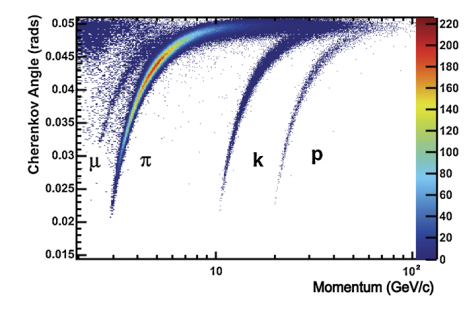
\includegraphics[width=0.49\linewidth]{figures/Chernkov_angle.PNG}
    \caption{Kaon identification efficiency and pion misidentification rate measured using simulated events as a function of track momentum. Two different $\Delta log \mathcal{L}(K − \pi)$ requirements (often called tight and loose) have been imposed on the
samples (left), reconstructed Cherenkov angle as a function of track momentum in the $C_4F_{10}$ radiator (right). Figures taken from \cite{RICH_performance}}%
    \label{fig:RICH_performance}%
 \end{center}
\end{figure}


\subsubsection{Muon Stations}

The proper muon identification is an essential requirement because muons are the final decay states of some of the most important heavy flavor decays such as $B_s^0 \rightarrow J/\psi ~~ \mu^{+}\mu^{-}$,  $B^{0}_s \rightarrow K^{*0} ~~ \mu^{+}\mu^{-}$ and they can be used as an initial flavor tag for measurements of $B^0$  and $B^0_{s}$ oscillations. 

The muon system provides muon identification as a log-likelihood variable, which depends on the track momentum and the number of hits detected in muon stations and how close the hits are with respect to the extrapolated track position in the muon system. It also provides such information as $x,y$ position in the muon station, which can be used for standalone-track reconstruction and finally $p_T$ information used by the L0 trigger system. More details refer to section \ref{sec:trigger}. Because the information from the muon stations is used in the hardware part of the LHCb trigger system, it is read out at the frequency of $40 Mhz$ (which is the LHC machine clock). 

Muon stations are located the farthest from the interaction point. The placement of these detectors is dictated by the fact that muons interact very weakly with the material, have a high masses ($105~ MeV/c^2$), and long lifetime ($2.2 \cdot 10^{-6}s$) thus muons travels much farther than any other charged particles.  
  
The muon system is composed of five stations, one situated just before the calorimeters and four downstream from them. Each of the stations is composed of two types of detectors. The first one is a multiwire proportional chamber located far from the beam pipe, and triple gas electron multiplier (GEM) detectors \footnote{GEM detector is used due to the higher particle flux} placed in central quadrants close to the beam. Those detector use gas mixture consisting of $Ar$, $CO_2$ and $CF_4$. A cartoon of the muon station is shown in figure \ref{fig:muon}. 
The efficiency of the muon identification is, on average, above $98\%$ with pion and kaon misidentification rate below $1\%$, which is shown in figure \ref{fig:muon_missidentify}. 


\begin{figure}[h]
 \begin{center}
  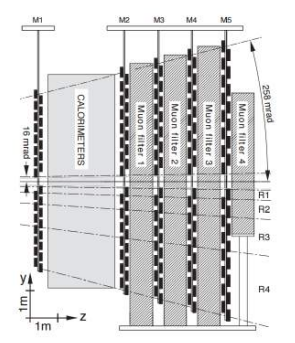
\includegraphics[width=0.49\linewidth]{figures/muon_stations.PNG}
   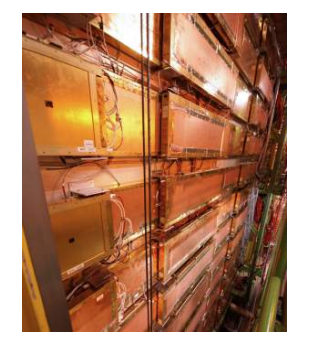
\includegraphics[width=0.49\linewidth]{figures/muon_photo.PNG}
    \caption{Side view of the muon detector (left) and a photo of M5 station. Figures taken from \cite{lhcb}.}%
    \label{fig:muon}%
 \end{center}
\end{figure}



\begin{figure}[h]
\centering
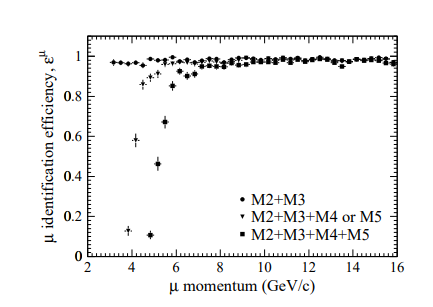
\includegraphics[scale=0.6]{figures/muon_eff.PNG}
\caption{Muon identification efficiency as a function of momentum, for different requirements on the number of hits. Figure taken from \cite{muon_tdr}.
\label{fig:muon_missidentify}}
\end{figure}



\subsubsection{Calorimeters}

The calorimeter system performs several functions. It is responsible for providing fast information for the hardware trigger level and allows identification of electrons, photons, and hadrons, jointly with a measurement of their energies and transverse positions.

The calorimeter system is designed to measure the energy of an interacting particle. This is achieved via measuring the energy of secondary electromagnetic and hadronic showers, which are created when a particle travels through the very dense absorber material (i.e., the material with a very low radiation length). The signal is formed using scintillator detectors (see text below). The measured energy is the total energy of all showers absorbed in the active materials, thus corresponds to the initial energy of the initial particle. 

The calorimeter system consists of an Electromagnetic Calorimeter (ECAL) and Hadron Calorimeter.  Both are placed between the first and second muon stations, see \ref{fig:LHCBlayout}. ECAL subdetector is dedicated to identifying photons and electrons.  It is equipped with two additional detectors, placed in front of it, a PreShower detector (PS) and a Scintillator Pad Detector (SPD), the layout and granularity of both are presented in figure \ref{fig:ECAL}. 

PS and the SPD are used by the low-level trigger to distinguish electrons from photons and pions. The information about the number of tracks per event obtained by SPD is also used by the trigger to drop events that are too busy. 
The ECAL is made of 2 mm lead plates followed by a 4 mm scintillator pad (shashlik like layout).  Its granularity depends on the distance from the beam, see figure \ref{fig:ECAL}.
The energy resolution of the ECAL detector can be expressed: 

\begin{equation}
    \frac{\sigma_{E}}{E} = \frac{10\%}{\sqrt{E/GeV}} \oplus     1 \%
\end{equation}
where: $\oplus $ denote addition in quadrature which can be formulated as: 
\begin{equation}
   \Delta a\oplus \Delta b = \sqrt{\Delta a^2 + \Delta b^2} 
\end{equation}


\begin{figure}
\centering
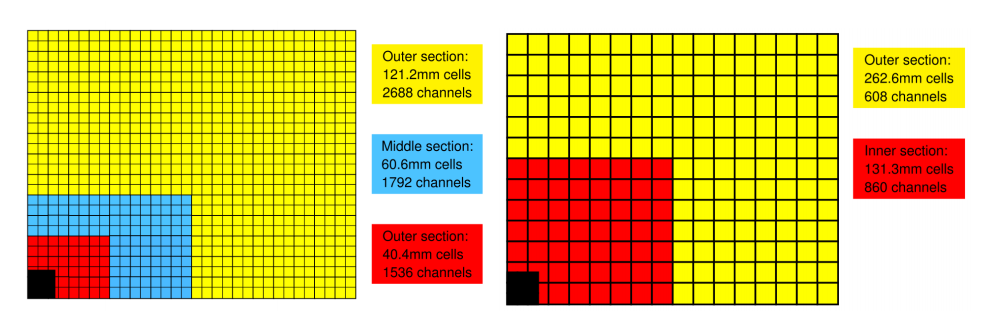
\includegraphics[width=\linewidth]{figures/ECAL.PNG}
\caption{Granularity for the different detector regions of the SPD, PS, and ECAL (left)
and of the HCAL (right). Figure taken from \cite{lhcb}.
\label{fig:ECAL}}
\end{figure}

The HCAL has an alternating structure of iron and scintillator tiles. The scintillator tiles are 4 mm tick and the iron ones are 16 mm. The HCAL energy resolution, obtained from the testbeam data can be expressed as: 

\begin{equation}
    \frac{\sigma_E}{E} = \frac{(69\pm 5) \%}{\sqrt{E}} \oplus (9\pm 2) \%
\end{equation}
 
\section{LHCb trigger}
\label{sec:trigger}
LHCb trigger is an example of the real-time system dedicated to compressing the input data stream. The raw data volume is far beyond the limit of the present storage technology, thus the necessity of employing such a system. The fundamental idea behind the large detector's trigger is to work out a decision whether a given event is interesting, from the point of view of the physics programme, or not. The LHCb trigger was designed to reduce the data rate from the initial bunch crossing rate of 40 MHz (i.e., one collision event each 25 ns) to about 12.5kHz of fully reconstructed events to be recorded on tapes. The data rate reduction is achieved by making a fast decision based on approximate measurement of particle transverse momentum and energy, muon identification, track displacement, and topological properties, which allows selecting some specific decays. 

The LHCb trigger is built as a two-stage system. The first one, called Level-$O$ trigger (or L$O$ for brevity), is implemented as a hardware layer with the fixed response time of 6 $mu s$. The processing power is provided by FPGA \footnote{FPGA stands for Field Programmable Gate Arrays, which are devices based on a matrix of configurable logic blocks. Their design has a benefit compared to a general-purpose CPU that allows massive parallelism since FPGA programable blocks can work independently and simultaneously as streaming processors.} chips. L$O$ trigger uses the information from calorimeters and muon stations to reduce the bunch-crossing rate to 1.1 MHz, which is the maximum input rate of the front-end ASICs used by other sub-systems. This partial information is then combined and process by dedicated electronics boards that give a final decision to process a given event further or drop it. 

%The L0 pileup triggers contribute to luminosity measurements \cite{trigger}.
The L$O$ calorimeter trigger leverage the information from ECAL, HCAL, PS, and  SPD detectors. Its decision is mostly based on transverse energy deposited in a cluster of $2\times 2$ cells (the cells are presented in figure \ref{fig:ECAL}) of the same size. The transverse energy, which is rather interesting quantity, is defined as:

\begin{equation}
    E_T = \sum_{i=1}^{4} E_i \sin\theta_i
\end{equation}

Where $E_i$ is the energy deposited in the $i-th$ cell, and $\theta_i$ is the angle between the beam axis and the direction of the particle's flight path. 
This quantity is combined with the information on the number of hits in the PS and SPD to distinguish between hadron, photon and electron candidates. 


Events accepted by the L0 trigger are sent to the Event Filter Farm, a computing cluster located at the LHCb pit, that consisted of approximately 29 000 and 50 000 CPU cores during Run 1 and Run 2 respectively. This computing farm is responsible for running High Level Trigger (HLT) application instances. The HLT software is written in C++ and consists of selection algorithms designed to identify specific decay processes, for instance, $b$ or $c$ hadron decays. The trigger strategy had changed over the course of years when LHCb detector collected the data. Figure \ref{fig:trigger} presents the triggering scheme for both Run 1 and Run 2. 


\begin{figure}
\centering
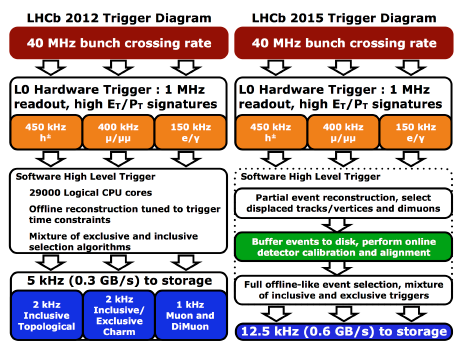
\includegraphics[width=\linewidth]{figures/trigger.PNG}
\caption{LHCb trigger data flow during Run 1 (left) and Run 2 (right). Each graph illustrate a high-level trigger architecture and a typical event acceptance rate after each stage. Figure taken from \cite{trigger_schame}.
\label{fig:trigger}}
\end{figure}

Implementing the second stage of the LHCb trigger as a full software application has
a great advantage of the flexibility that plays a paramount role in adapting to changing
data taking conditions. On the other hand, it also requires constant monitoring of the
trigger configuration, which is a highly non-trivial task. The machine provided beams
that were tuned in the way that the average number of proton-proton interactions per
one beam crossing was 1.6. The data taking periods, when protons were circulating
in the machine, were called fills and they were, in turn, divided in runs. Each run
could possibly be configured individually, taking into account differences in the Data
Acquisition system, calibration and alignment conditions etc. 

%HLT consists of two stages, the first one called HLT1 evaluates a simplified version of tracking and muon reconstruction in order to identify the track that could trigger an event quickly. HLT1 allows reducing the data flow going from the L0 trigger, giving a sufficient amount of time to HLT2 to perform the more sophisticated reconstruction.

During the down period between Run 1 and Run 2 (called the Long Shutdown 1) a considerable amount of work has been done to optimise and improve the HLT software. This led to splitting the trigger into two logically exclusive parts called HLT1 and HLT2 (see text below for details). It allowed evaluating the online alignment and calibration, while the events were stored in the disk buffer.
The online calibration procedures were vital for achieving high-quality reconstruction in HLT that is comparable to the offline one.

Within HLT1 the full detector information is used. The reconstruction process starts with the vertex detector. The track candidates are selected based on the probability that particular track originates from heavy flavor decay, which is achieved by determining their impact parameter. Selected tracks are then associated with track segments in the tracking stations, which allows estimation of the transverse momentum of the corresponding charged particle (so called forward tracking algorithm). This information, together with track's $\chi^2$ and impact parameter $\chi^2_{IP}$, is used to select interesting events.  
During Run 2, a small portion of data selected by HLT1 was used to calibration and alignment of the detectors. This process, which takes a few minutes, is performed to reduce the probability of misalignment on the tracker. Any misalignment would impact the momentum resolution affecting the quality of reconstruction in HLT2. No particle-identification is available at this stage (apart from a coarse muon identification). The final output rate of HLT1 is approximately 110 kHz.

The final selections are performed by HLT2 trigger using the full particle identification variables. HLT2 implements two types of trigger lines that select exclusive and inclusive processes, respectively . Exclusive algorithms are used to select specific decays. For instance, they required all decay products to be within the detector acceptance and reconstructed. 
Inclusive trigger selections, also called topological lines, trigger on partially-reconstructed $b$ hadrons decays. Those lines are designed to detect all $b$ hadrons decays with a displaced secondary vertex, and at least two charged particles in the final state. The output bandwidth is divided into three streams and undergoes constant, careful monitoring. About 40$\%$ of the total output rate is assigned to inclusive topological selections, another 40$\%$ is reserved to exclusive lines targeting the c-hadron decays and the rest is given to other exclusive processes.
The quality of reconstruction in the HLT2 during Run 2 allowed LHCb to implement so-called "Turbo" lines that return fully reconstructed analysis-ready data. Additionally, those lines allow saving space by discarding the raw data, keeping only the relevant information describing reconstructed events. 

The trigger efficiency is estimated using the so-called TIS-TOS (Triggered Independent of Signal - Triggered on Signal) method, described in detail in \cite{trigger_eff}. TOS events are those where daughter particles that form a particular decay candidate passed the trigger selection criteria. In the case where other particles in the event passed the criteria, a given decay candidate is called TIS.
Both categories are not exclusive. When estimating the trigger efficiency, detailed knowledge of which class a given event belongs to is very important.
It should be stressed that the reconstruction algorithm that is the subject of this thesis (described in chapter \ref{chapter:PLLT}) was executed as a part of the HLT2. 

\section{LHCb software}

In order to produce the Monte Carlo simulated samples (see figure \ref{fig:lhcb_sim}) and analyze data collected by the LHCb spectrometer a dedicated software framework has been designed and implemented \cite{lhcb_software}. Most of the applications were written in  C++, and they are based on two frameworks ROOT \cite{root} and Gaudi \cite{gaudi}. The list below contains a brief description of selected packages:

\begin{itemize}
    \item \textbf{Gauss} \cite{gauss_lhcb} was designed to generate the initial particles and simulates their transport through the LHCb detector. The Gauss application consists of two major independent processing phases. The first one is a generation of the proton-proton interactions (primary vertices), at LHC energies, that result, in turn, in producing primary particles. This generation process  is handled by PYTHIA \cite{pythia}, a general-purpose event generator, whist the decay and time evolution of the produced particles is delegated to EventGen \cite{EventGen}. The second phase of Gauss application performs detector response simulation via a customized Geant4 \cite{geant4} based module. 
    \item \textbf{Boole} \cite{lhcb_software}  performs a final stage of the LHCb detector simulation. It applies the detector response to hits previously generated by the Gauss. This step, called digitization, includes simulation of the detector and read-out electronics response, together with L0 trigger hardware information. The output format of Boole corresponds exactly to the data coming from the real detector.
    \item \textbf{Brunel} \cite{lhcb_software} this package is responsible for the whole process of data reconstruction, which consist of retrieving all recorded hits in a detector, doing the pattern recognition to identify trajectories, finding primary vertices of proton-proton interactions, and assigning PID likelihoods. Brunel can process both simulated and the real collected by detector data in a completely agnostic way. The outcome of the Brunel consists of the high-level reconstructed objects (e.g tracks and vertices described in Chapter~\ref{chapter:PLLT}) that are saved in a Data Summary Tape (DST) format.   
    \item  \textbf{DaVinci} \cite{lhcb_software} was designed to process the Brunel output and, based on it, reconstruct decays of interest and apply selection criteria to reduce the background. The outcome of this step is a dataset containing decay candidates for the user-specific decay topologies, which are used as a starting point for further physics analyses.   
    
\end{itemize}


\begin{figure}[!h]
\centering
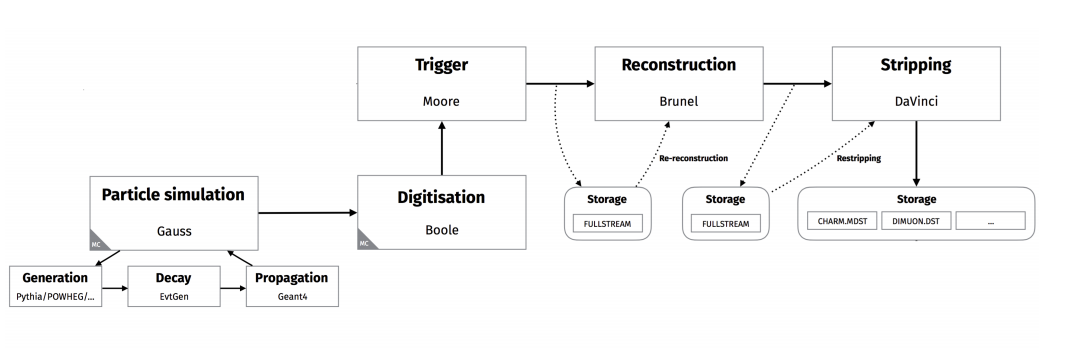
\includegraphics[angle =90]{figures/LHCb_simulation.PNG}
\caption{LHCb event simulation flowchart. Each rectangle with a sharp corners represents a separated LHCb package described in text. Figure taken from  \cite{lhcb_computing}.
\label{fig:lhcb_sim}}
\end{figure}



\section{LHCb upgrade}
This section is divided into three parts. The first one is dedicated to present the general concepts of why LHCb collaboration decided to upgrade its detector. The second one describes the scope of the Upgrade by discussing which elements will be replaced. The final subsection focuses on the Upstream Tracker detector. It provides a very detailed description of this detector since the author was personally involved in its development.  

\subsection{Motivation}

The data collected during both Run 1 and Run 2 allowed to perform and report several World best measurements of rare decays of $b$ and $c$ hadrons, which were used to set new limits on models describing New Physics. However, many measurements are still limited by the statistical uncertainties. Continuing data collection at the current rate would not allow us to decrease them to the level compatible with the theoretical predictions. In order to increase annual data yields, the LHCb detector must undergo a major upgrade during the Long Shutdown 2 (expected to be finished in early 2022).  The changes will allow the detector to operate at the increased luminosity of $20 \times 10^{33} cm^{-2}s^{-1}$, which is five times higher than the previous one. The new detector is expected to read data (full detector information) at the bunch crossing rate of 40 MHz, which allows collecting about $10~ fb^{-1}$ per year while during both Run 1 and Run 2, LHCb collected approximately $8~ fb^{-1}$. Figure \ref{fig:lhcb_lumi} present the luminosity plan. This figure also presents the prediction of the longer-term future of the LHCb experiment, which is out of the scope of this thesis.  

\begin{figure}[!h]
\centering
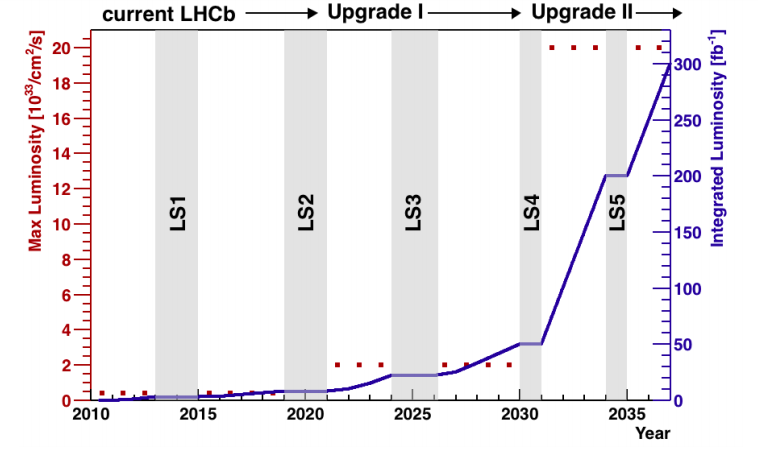
\includegraphics[width=\linewidth]{figures/lhcb_lumi.PNG}
\caption{Actual and predicted integrated luminosity from 2010 to 2037 for the LHCb experiment. Red dots represent
the value of measured or predicted instantaneous luminosity. Solid blue line represents the value of measured or predicted integrated luminosity.
\label{fig:lhcb_lumi}}
\end{figure}


\subsection{General aspects of the LHCb Upgrade}

One of the main limitations that drive the idea of the LHCb Upgrade was the limitation of the hardware L$O$ trigger and the readout electronics (which resulted in limited event input rate to HLT trigger). This limitation comes from the specific of the current read-out system, see section \ref{sec:velo}.  To overcome this limitation, all tracking detectors and their read-out systems have to be replaced to be capable of reading out the full detector information at the rate of $40 ~MHz$. New read-out electronics will allow removing the L0 trigger, keeping only the software flexible part. Figure \ref{fig:lhcb_upgrade} presents the new layout of the LHCb detector. When comparing this layout with the previous one, see figure \ref{fig:LHCBlayout}, it is clearly visible that the overall structure of the spectrometer stays as it was. All components of the tracking system (vertex detector, TT and T stations) will be replaced. The Cherenkov detectors will be heavily modified, and both the PS and SPD detectors will be removed from the spectrometer. Only the detectors that were previously contributing to the L0 trigger will not have major interventions. 

\begin{figure}[!h]
\centering
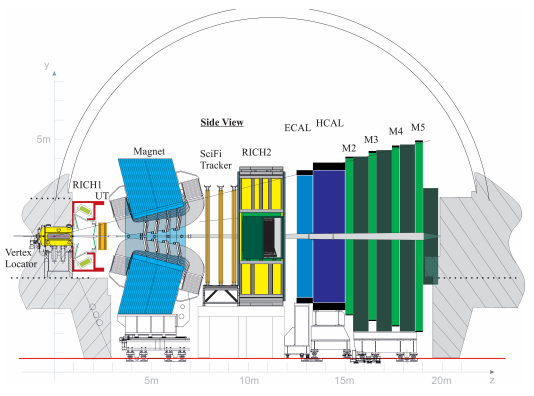
\includegraphics[width=\linewidth]{figures/LHCb_upgrade.PNG}
\caption{Layout of the upgraded LHCb detector. Figure taken from \cite{upgrade_tracker_tdr}
\label{fig:lhcb_upgrade}}
\end{figure}

\subsection{Upgraded Velo}
The upgraded Velo detector will be placed closer to the beam, its active area will reach the distance of $5.1 mm$ from the beam axis, and it will have a finer granularity thanks to changing from micro-strip to pixel technology. The new Velo will operate at much higher particle flux due to increased luminosity, which causes an increase in the average number of visible proton-proton collisions from 1.6 to 5.2 (i.e., on average 5.2 primary vertices will be present at each beams crossing). Thus, the Velo group decided to use pixel sensors to reduce occupancy. The upgraded Velo detector will consist of 41 million $55\times 55 \mu m$ pixels, which will be read out by the custom-build VeloPix front-end ASIC, at the 40 MHz rate. 
The cooling is provided by evaporative $CO_{2}$ system. It will employ an innovative micro-channels embedded in the structure of the support silicon modules.
A layout of the upgraded Velo module is shown in figure \ref{fig:veloUpgradeModule}. 
Both the expected performance of the track reconstruction efficiency and impact parameter as a function of the inverse of the transverse momentum are shown in figure \ref{fig:upgrade_velo_performance}.    

\begin{figure}[!h]
\centering
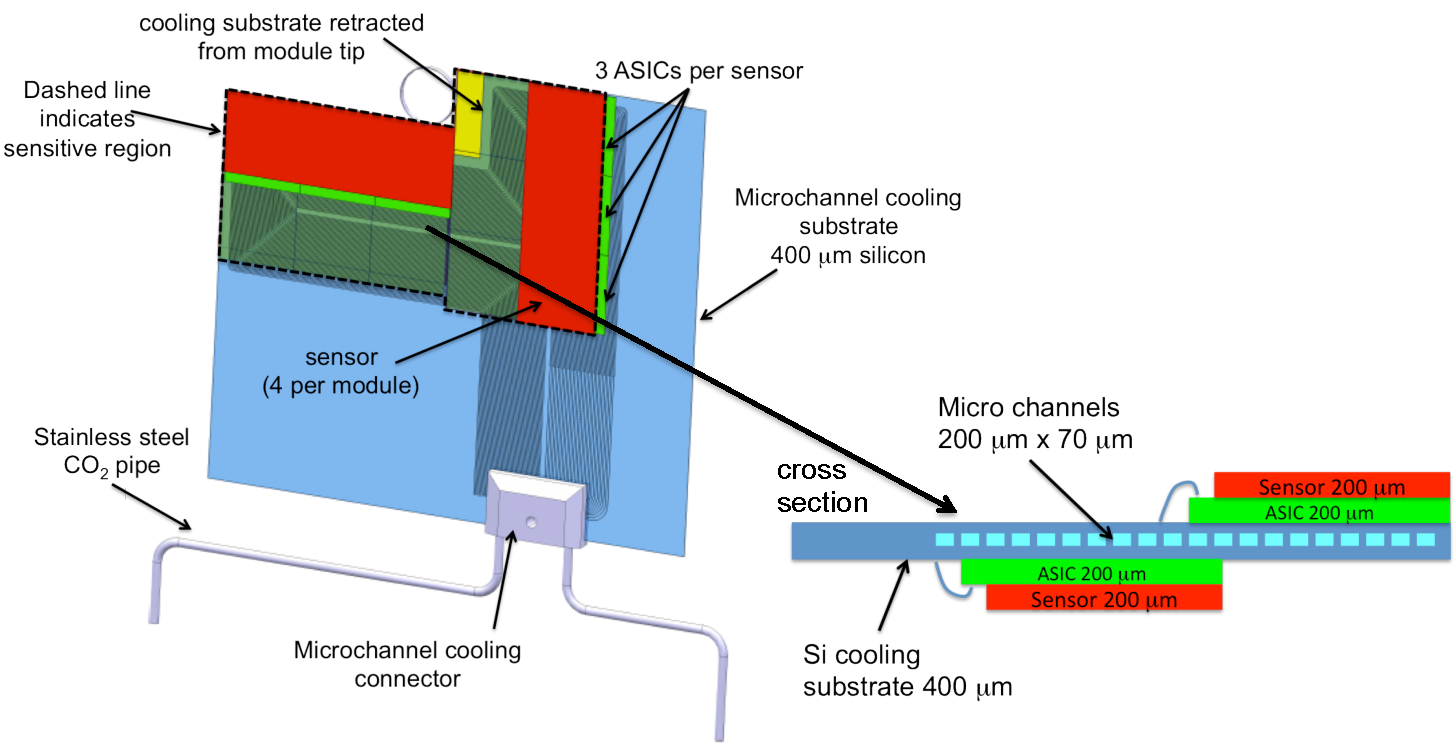
\includegraphics[width=\linewidth]{figures/Velo_upgraded_module.pdf}
\caption{Layout of a module of the upgraded VELO detector. Figure taken from \cite{velo_upgrade_tdr}
\label{fig:veloUpgradeModule}}
\end{figure}




\begin{figure}[!h]
 \begin{center}
  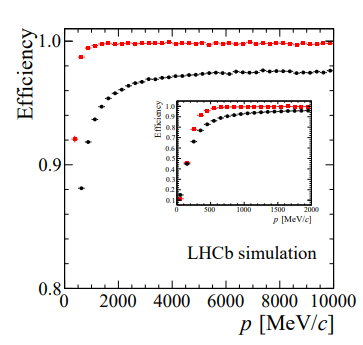
\includegraphics[width=0.49\linewidth]{figures/Velo_upgrade_tracking.PNG}
   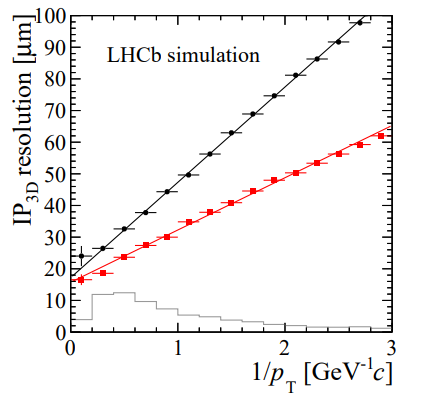
\includegraphics[width=0.49\linewidth]{figures/Velo_upgrade_IP.PNG}
    \caption{The left figure shows the reconstruction efficiency evaluated for particles which are reconstructible as Velo tracks as a function of momentum. The right plot shows the  3D resolution of the IP, the light gray histogram shows the relative population of $b$ hadron daughter tracks in each $1/p_t$ bin. Figures taken from \cite{velo_upgrade_tdr}.}%
    \label{fig:upgrade_velo_performance}%
 \end{center}
\end{figure}

\subsection{Scintillating Fibre Tracker}

Scintillating Fibre Tracker (FT) \cite{upgrade_tracker_tdr} \footnote{The previous name of this sub-detector was SciFi and referred to the speculative fiction genre since many people did not believe that the construction of such a detector is feasible.} was designed to replace the T tracking stations. Two factors drove this decision. Extensive simulations studies showed that the upgraded condition would be too harsh for a straw gas detector (like the previous OT gaseous system). The foreseen occupancy would be too high to provide reliable input to the tracking pattern recognition algorithm. Moreover, the readout electronics of both OT and IT detectors would not be capable of working as a part of a new data acquisition system. FT tracker covers the full LHCb detector acceptance downstream to the magnet and, by design, guarantees a spatial resolution close to $80 \mu m$. 
This detector will consist of three stations, each of them composed of four detection planes organized, similar to IT,  in a $(X, U, V, X)$ orientation, see figure \ref{fig:SciFI}.
 The module will consist of scintillating fibres with a radius of  $125 \mu m$, and a length of 2.5 m, which will be read out by Silicon Photo-Multipliers (SiPMs), located either at the top or bottom of the detector. The SiPMs are kept in a cold box, at $-40 \circ C$, to reduce the dark count rate \footnote{The dark count rate, is the count rate that is measured in the absence of photons, is caused by thermally generated electron-hole pairs.}, and each of them consists of nearly 128 individual pixels.   


\begin{figure}[!h]
\centering
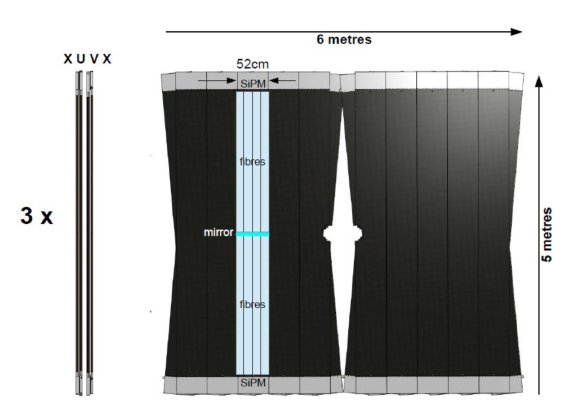
\includegraphics[scale=0.6]{figures/SciFi.PNG}
\caption{Layout of one tracking station of the SciFi detector. Figure taken from \cite{upgrade_tracker_tdr}
\label{fig:SciFI}}
\end{figure}

The FT detection mechanism is based on measuring the photons emitted when a particle traverses the detector's active area. Those photons are propagated through the fibres and finally reach the silicon pixels located at the end of the fibres. A signal proportional to the number of photons detected within a given SiPM detector is used to determine the position of the particle, shown in figure \ref{fig:SciFI_idea}. Each pixel can detect one photon at a time.


\begin{figure}[!h]
\centering
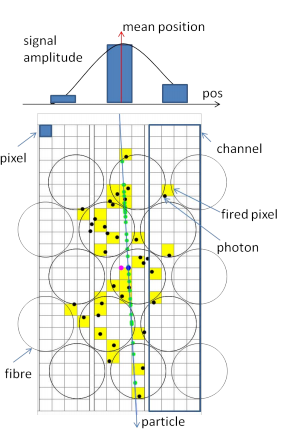
\includegraphics[scale=0.5]{figures/SciFi_idea.PNG}
\caption{Simplified visualization of the detection mechanism of the FT. The squares show the pixels located at the end of the fibres, and the circles indicate the cross-section of the scintillating fibres. Note that the fibres are not aligned to the detector channels, and the photons can arrive at the detector outside the fibre area.  Figure taken from \cite{upgrade_tracker_tdr}
\label{fig:SciFI_idea}}
\end{figure}

 
 \section{Upstream Tacker}
 \label{sec:UT}
The Upstream Tracker (UT) is a detector that was designed to replace TT tracker. Its structure and sensor technology is very similar to its predecessor. Thus it will be composed of four planes of silicon-strip detectors divided into two stations, as it is schematically shown in figure \ref{fig:UT_scheme}. Similarly to TT, the detector plates will be arranged in a $(X, U, V, X)$ orientation, with the second and third planes rotated at a stereo angle of $\pm5^{\circ}$ with respect to the $y$-axis.   

 \begin{figure}[!h]
\centering
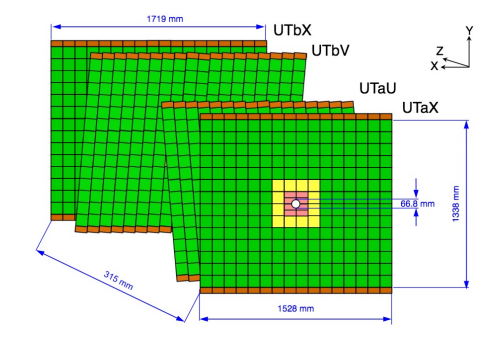
\includegraphics{figures/UT.png}
\caption{Layout of the four UT detector planes (looking downstream of the interaction point). Outermost, intermediate, and innermost sensors are shown in green, yellow, and reddish, respectively. Figure taken from \cite{upgrade_tracker_tdr}
\label{fig:UT_scheme}}
\end{figure}


The expected trigger efficiency enhancement with respect to the TT will originate from improved acceptance coverage at small polar angles and finer granularity.  This will be achieved by designing the innermost sensor to have a circular cut-off around the beampipe, as shown in figure \ref{fig:UT_scheme} (reddish sensors). The UT sensors will have improved radiation hardness, which is critical since the UT sensors have to withstand an integrated luminosity of $50~ fb^{-1}$, which is a factor of 5 more than TT.  Figure \ref{fig:UT_dose} presents  the expected irradiation dose, estimated by a FLUKA simulation \cite{fluka}, after $50~ fb^{-1}$ as a function of $y$ coordinate, obtained for a detector station slice at $x=0$. Those expected irradiation doses drove the decision on the sensor's technologies. The sensors that are situated closer to the beam will be $n^{+}\text{-on-p}$ technology, which is more radiation hard than $p^{+}\text{-on-n}$.  
 
 \begin{figure}[!h]
\centering
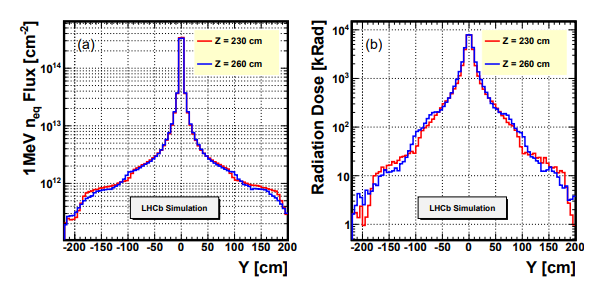
\includegraphics{figures/UT_dose.PNG}
\caption{Expected fluence profile (left) and radiation dose profile (right) as a function of $y$-coordinate, for a slice of the detector that is positioned at $x=0$. This slice represent the highest fluence region throughout the UT system. Figure taken from \cite{upgrade_tracker_tdr}
\label{fig:UT_dose}}
\end{figure}

 
 Four different sensors geometries, denoted type-A, B, C, and D, are used in the UT detector depending on proximity to the beam pipe, see figure \ref{fig:UT_sensors}. To mitigate the effects of irradiation and reduce leakage current, the cooling system is designed to provide a maximum operating temperature of the silicon detectors of $-5\circ C$. 
 
 
 
 \begin{figure}[!h]
\centering
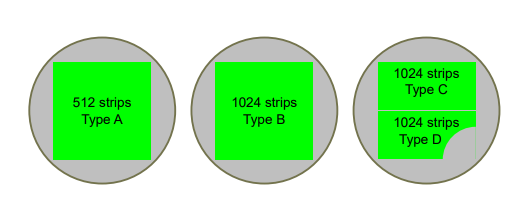
\includegraphics{figures/UT_sensors.PNG}
\caption{Sketch of the three mask designs for the UT upgrade. Sensors C and D are shorter and
can be produced in a single 4-inch wafer, whereas sensors A and B require a full wafer.  Figure taken from \cite{upgrade_tracker_tdr}
\label{fig:UT_sensors}}
\end{figure}
 
 \section{SALT ASIC}
 \label{sec:salt}
The design of the new strip readout chip, operating at bunch crossing frequency of 40 MHz, was a critical part of the LHCb Upgrade. The primary goal of this ASIC was to overcome hardware trigger limitation, which significantly limited the amount of collected data in Run 1 and Run 2, see section \ref{sec:trigger}. 
The Silicon ASIC for LHCb Tracking (SALT) is a chip designed at AGH-UST Krakow that is capable of reading 128-channels. It was manufactured in radiation-hard TSMC CMOS\footnote{CMOS stands from Complementary metal–oxide–semiconductor and it's a technology that uses complementary and symmetrical pairs of p-type and n-type  MOSFETs (Metal–Oxide–Semiconductor Field-Effect Transistor) for logic functions.} $130 nm$ \footnote{$130 nm$ refers to the minimum gate length that can be manufactured using a particular technology. } technology and employed a novel architecture comprising an analogue front-end and an ultra-low power (< 0.5 mW) fast (40 MSps\footnote{milion of samples per second}) sampling 6-bit ADC in each channel. Thus, the chip is capable of performing quite involved data processing on-detector and significantly reducing the data volume sent to the trigger system.


\begin{figure}[ht!]
\centering
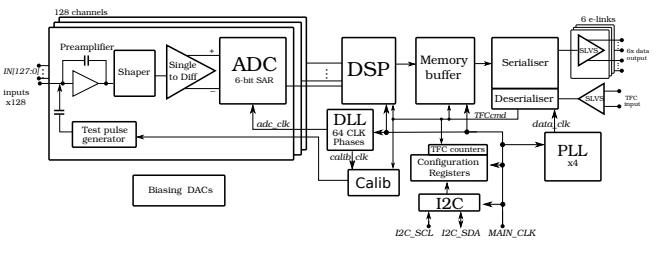
\includegraphics{figures/SALT_2.PNG}
\caption{Block diagram of the SALT ASIC readout chip, see text for more details. Figure taken from \cite{SALT}.
\label{fig:SALT}}
\end{figure}


The Salt consists of two main blocks analog and digital, see diagram \ref{fig:SALT}. The analog block consists of a charge preamplifier and a fast shaper with a peaking time of about $25 ns$, and 25 ns after the peaking time of no more than $5\%$ of the peak value.  Those parameters are required to distinguish between consecutive LHC bunch crossings. The SALT was designed to operate with both types ($p^{+}\text{-on-n}$ and $n^{+}\text{-on-p}$) of strip sensors with capacitance in range $5-20~ pF$. 
The shaper is followed by a single-to-differential block that converts a single-ended signalling to a differential one \footnote{Single-ended signaling is a method of signal transmission where one wire carries a changing voltage (signal) and the second wire is connected to a reference voltage (ground), while differential signaling sends a signal via employing two complementary voltage signals to transmit one information signal \cite{signals}}. The last component of the analog block is a fully differential 6-bit SAR ADC, which converts the analog signal to the digital domain. 

The digital ADC output is processed by a Digital Signal Processing (DSP) block, which performs the following algorithms: 

\begin{itemize}
    \item \textbf{Channel masking}. Noisy or dead channels can be masked and removed from further processing; 
    \item \textbf{Pedestal subtraction}. This subtraction is performed in each channel independently using a different value;
    \item \textbf{Mean Common Mode Subtraction}. Removal of the mean value of calculated on top of channels with signal below the certain hit threshold; 
    \item \textbf{Zero Suppression}; Only the data registered in channels where the signal is above hit threshold are sent out for further processing in the trigger system.
\end{itemize}

Since high level emulation of these algorithms is part of the topic of this thesis, the detailed explanation of each can be found in chapter \ref{chapter:tbut}. 

After the DSP, the data is serialized and sent out through, so-called, e-links using SLVS interface \cite{SLVS} operating at $320 MBit/s$ data rate. Each ASIC is equipped with  e-links, but only some of them are active, depending on the expected hit occupancy on the sensor.  The configuration and monitoring of the SALT ASIC can be adjusted through the Inter-Integrated
Circuit ($I^{2}C$) interface \cite{i2c}.  

